\documentclass[14pt]{article}

\usepackage[utf8x]{inputenc}
\usepackage[russian]{babel}
\usepackage{graphicx}
\graphicspath{{images/}}
\DeclareGraphicsExtensions{.pdf,.png,.jpg}

\usepackage{amsmath}
\usepackage{multirow}
\usepackage{pgfplots}

\usepackage{geometry} % Меняем поля страницы
\geometry{left=2cm}% левое поле
\geometry{right=1.5cm}% правое поле
\geometry{top=2cm}% верхнее поле
\geometry{bottom=2cm}% нижнее поле

\renewcommand{\theenumi}{\arabic{enumi}}% Меняем везде перечисления на цифра.цифра
\renewcommand{\labelenumi}{\arabic{enumi}}% Меняем везде перечисления на цифра.цифра
\renewcommand{\theenumii}{.\arabic{enumii}}% Меняем везде перечисления на цифра.цифра
\renewcommand{\labelenumii}{\arabic{enumi}.\arabic{enumii}.}% Меняем везде перечисления на цифра.цифра
\renewcommand{\theenumiii}{.\arabic{enumiii}}% Меняем везде перечисления на цифра.цифра
\renewcommand{\labelenumiii}{\arabic{enumi}.\arabic{enumii}.\arabic{enumiii}.}% Меняем везде перечисления на цифра.цифра

\begin{document}
\begin{titlepage}
	\begin{center}
		\fontsize{18pt}{20pt}\selectfont
		\textbf{Работа 1.2.5.}	
	
		\vspace{5cm}
		\fontsize{24pt}{25pt}\selectfont
		Исследовании прецессии уравновешенного гироскопа
	\end{center}
	\begin{flushright}
		\fontsize{18pt}{20pt}\selectfont
		\vspace{14cm}
		\hspace{-3cm}
		\textit{Корнеев Е.С.}
	\end{flushright}		
\end{titlepage}

\begin{center}
	\fontsize{16pt}{18pt}\selectfont	
	Исследовании прецессии уравновешенного гироскопа
\end{center}

\fontsize{14pt}{16pt}\selectfont
\vspace{1cm}
\textbf{Цель работы:} исследовать вынужденную прецессию гироскопа; установить зависимость скорости вынужденной прецессии от величины момента сил, де	ствующих на ось гироскопа; определить скорость вращени ротора гироскопа и сравнить ее со скоростью, рассчитанной по скорости прецессии.

\vspace{0.5cm}
\textbf{В работе используются:} гироскоп в кардановом подвесе, секундомер, набор грузов, отдельный ротор гироскопа, цилиндр известной массы, крутильный маятник, штангенциркуль, линейка.

\vspace{1cm}
Уравнение движения твердого тела можно записать в виде

\begin{equation}
\frac{d\vec{P}}{dt} = \vec{F}
\end{equation}

\begin{equation}
\frac{d\vec{L}}{dt} = \vec{M}
\end{equation}

Здесь (1) выражает закон движения центра масс тела, а (2) --- уравнение моментов. Поскольку твердое тело имеет только шесть степеней свободы, этих двух векторных уравнений достаточно для полного опиcания состояния движения.

Если сила $\vec{F}$ не зависит от угловой скорости, а момент $\vec{M}$ --- от скорости поступательного движения, то уравнения (1) и (2) можно рассматривать независиъмо друг от друга. В баллистике, например при движении снаряда в воздухе, это невозможно. В случае же, когда такое раздельное рассмотрение возможно, уравнение (1) соответствует просто задаче о движении материальной точки, а уравнение (2) --- задаче о вращении твердого тела вокруг неподвижной точки. В данной работе рассматривается последняя из этих задач.

Момент импульса твердого тела в его главных осях $x, y, z$ равен

\begin{equation}
\vec{L} = \vec{i}I_x\omega_x + \vec{j}I_y\omega_y + \vec{k}I_z\omega_z
\end{equation}

\noindent где $I_x, I_y, I_z$ --- главные моменты инерции, $\omega_x, \omega_y, \omega_z,$ --- компоненты вектора угловой скорости 
$\vec{\omega}$. Быстро вращающееся тело, для которого, например,

$$I_z\omega_z \gg I_x\omega_x, I_y\omega_y$$

\noindent принято называть гироскопом. Гироскоп называтся уравновешенным, если его центр масс неподвижен.

В силу (2) приращение момента импульса определяется интегралом

\begin{equation}
\Delta \vec{L} = \int\vec{M}dt
\end{equation}

\noindent Если момент внешних сил действует в течение короткого промежутка времени, из интеграла (4) следует, что приращение $\Delta\vec{L}$ момента импульса значительно меньше самого момента импульса:

\begin{equation}
|\Delta\vec{L}| \ll |\vec{L}|
\end{equation}

\noindent С этим связана замечательная устойчивость, которую приобретает движение гироскопа после приведения его в быстрое вращение.

\begin{figure}[h!]
	\center{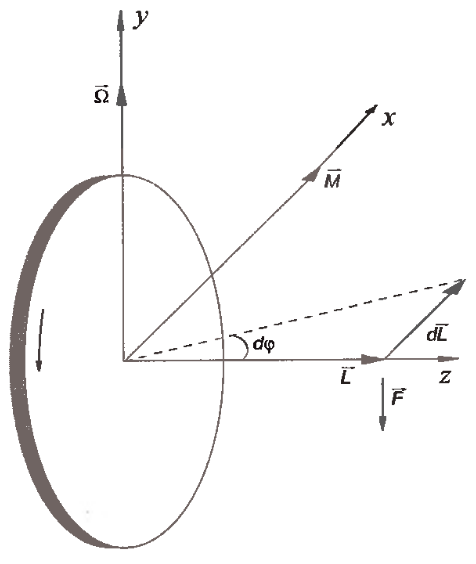
\includegraphics[width = 6cm]{flywheel}}
	\caption{Маховик}
	\label{fig:image}
\end{figure} 

Выясним, какие силы надо приложить к гироскопу, чтобы изменить направление его оси. Рассмотрим для примера маховик, вращающийся вокруг оси $z$, перпендикулярной и к плоскости маховика (рис. 1). Будем считать, что

$$\omega_z = \omega_0, ~~~\omega_x = 0, ~~~\omega_y = 0.$$

\noindent Пусть ось вращения повернулась в плоскости $xz$ по направлению к оси $x$ по направлению к оси $x$ на $d\varphi$. Такой поворот означает добавочное вращение маховика вокруг оси $y$, так что 

$$d\varphi = \Omega dt,$$

\noindent где $\Omega$ --- угловая скорость такого вращения. Будем предполагать, что 

\begin{equation}
L_{\Omega} \ll L_{\omega_0}
\end{equation}

\noindent Это означает, что момент ипульса маховика, равный $I_z\omega_0$ до приложения внешних сил, только повернется в плоскости $zx$ по направлению к $x$, не изменяя величины. Таким образом,

$$|d\vec{L}| = Ld\varphi = L\Omega dt$$

\noindent Но это изменение направлено против оси $x$, поэтому вектор $d\vec{L}$ можно представить в видевекторного произведения вектора угловой скорости $\vec{\Omega}$, направленного противо оси $y$, на вектор собственного момента импульса маховика, направленного вдоль оси $z$,

$$d\vec{L} = \vec{\Omega} \times \vec{L}dt,$$

\noindent т.е.

$$\frac{d\vec{L}}{dt} = \vec{\Omega} \times \vec{L}$$

\noindent В силу (2) имеем

\begin{equation}
\vec{M} = \vec{\Omega} \times \vec{L}
\end{equation}

\noindent Формула (6) справедлива, если выполнено условие (5). Она позволяет определить момент сил $\vec{M}$, который необходимо приложить к маховику для того, чтобы вызвать вращение оси маховика с угловой скоростью $\vec{\Omega}$. Мы видим, таким образом, что для поворота оси вращающегося маховика к оси $x$ необходимо приложить силы, направленные не вдоль оси $x$, а вдоль оси у, так чтобы их момент $\vec{M}$ был направлен вдоль
оси $x$.

Под действием момента $\vec{M}$ внешних сил ось гироскопа медленно вращается вокруг оси $y$ с угловой скоростью $\Omega$. Такое движение называется регулярной прецессией гироскопа. В частности, создающей момент внешней силой может оказаться сила тяжести, если центр масс гироскопа не совпадает с точкой подвеса. Для гироскопа массой $m_{\text{г}}$, у которого ось собственного вращения наклонена на угол $\alpha$ от вертикали, скорость прецессии, происходящей вокруг вертикальной оси под действием силы тяжести, равна

\begin{equation}
\Omega = \frac{M}{I_x\omega_0\sin\alpha} = \frac{m_{\text{г}}gl_{\text{ц}}\sin\alpha}{I_x\omega_0\sin\alpha} = \frac{m_{\text{г}}gl_{\text{ц}}}{I_x\omega_0}
\end{equation}

\noindent где $l_{\text{ц}}$ --- расстояние от точки подвеса до центра масс гироскопа, т. е. скорость прецессии не зависит от угла $\alpha$. 

Для изучения регулярной прецессии уравновешенного гироскопа к его оси подвешивают дополнительные грузы. Это смещает общий центр масс и создает момент сил тяжести, вызывающий процессию. Скорость прецессии в этом случае равна

\begin{equation}
\Omega = \frac{mgl}{I_x\omega_0},
\end{equation}

\noindent где $m$ --- масса груза, $l$ --- расстояние от центра карданова подвеса до точки крепления груза на оси гироскопа (рис. 3).

В данной работе исследуется регулярная прецессии уравновешенного гироскопа.

Уравновешенный гироскоп, закрепленный в кольцах карданова подвеса, показан на рис. 2. Наружное кольцо подвеса А может свободно поворачиваться вокруг вертикальной оси $aa$. Внутреннее кольцо Б связано с кольцом А горизонтальной осью $\text{бб}$. В кольце Б укреплен гироскоп, ось вращения которого $\text{вв}$ перпендикулярна к оси $\text{бб}$. Центр масс гироскопа находится на пересечении всех трех осей и при любом пово-
роте колец сохраняет свое положение в пространстве. Получается, что гироскоп как бы подвешен за центр масс.

\begin{figure}[h!]
	\center{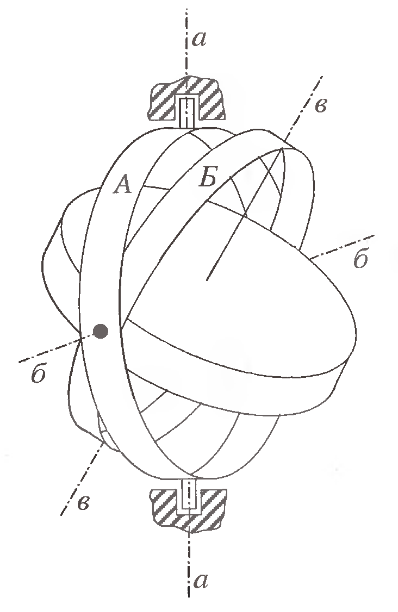
\includegraphics[width = 6cm]{gyro}}
	\caption{Гироскоп в кардановом подвесе}
	\label{fig:image}
\end{figure} 

Экспериментальная установка для исследования прецессии уравновешенного гироскопа показана на рис. 3. Ротором гироскопа является ротор высокооборотного электромотора М, питающегося током частотой 400 Гц. Кожух мотора (статор. имеющий обмотки, питаемые током частотой 400 Гц) скреплен с кольцом Б (рис. 2 и 3). Мотор с кольцом Б может вращаться в кольце А вокруг горизонтальной оси $\text{бб}$, которое может вращаться вокруг вергикальной оси $\text{аа}$. Ротор электромотора представляет массивный стальной цилиндр с прожилками меди, образуюпшми «беличье колесо». Обозначенный на рис. 3 буквой С рычаг направлен по оси симметрии ротора. На рычаг подвешивают грузы Г. Подвешивая раапичные грузы, можно менять силу $F$, момент которой определяется расстоянием $l$ от точки педвеса до горизонтальной оси кольца А (до центра масс гироскопа), указанным на самой установке.

Выше при выводе формул для прецессии предполагалось, что действующие на гироскоп силы лежат в плоскости $xy$, в которой лежат векторы угловых скоростей собственною вращения и прецессии. В этом случае, как уже говорилось, момент сил меняет лишь направление момента импульса гироскопа, но не его величину. Силы трения не лежат в плоскости осей вращения. Они приводят к изменению момента импульса и по направлению, и по величине. Для ротора гироскопа действие сил трения скомпенсировано действием электромотора. Для осей карданова подвеса компенсации нет. В результате ось гироскопа будет опускаться в направлении действия груза. 

\begin{figure}[h!]
	\center{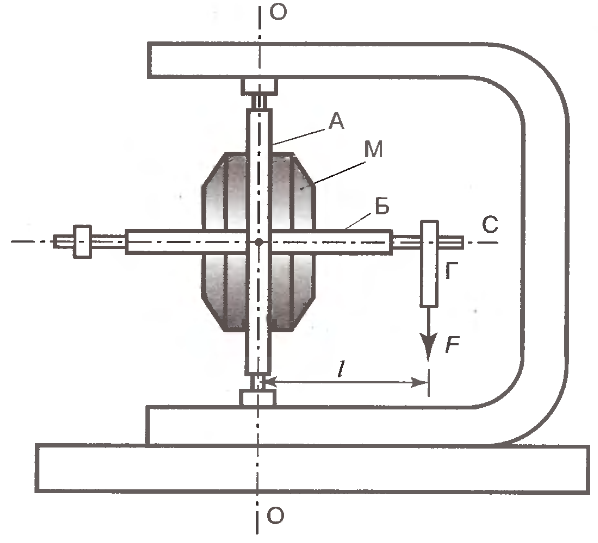
\includegraphics[width = 9cm]{scheme}}
	\caption{Схема установки}
	\label{fig:image}
\end{figure} 

В первой части работы исследуется зависимость скорости прецессии гироскопа от момента силы, приложенной к его оси. Для этого к оси гироскопа (к рычагу С) подвешиваются грузы Г. Скорость прецессии определяется по числу оборотов рычага вокруг вертикальной оси и времени, которое на это ушло, определяемое секундомером. В процессе измерений рычаг не только поворачивается в результате прецессии гироскопа, но и опускается. Поэтому его в начале опыта следует приподнять на $5-6^{\circ}$ . Опыт надо закончить, когда рычаг опустится на такой же угол.

Измерение скорости прецессии гироскопа позволяет вычислить угловую скорость вращения его ротора. Расчет производится по формуле (8). Момент инерции ротора относительно оси симметрии и измеряется по крутильным колебаниям точной копии ротора, подвешиваемой вдоль оси симметрги на жесткой проволоке. Период крутильных колебаний $T_0$ зависит от момента инерции $I_0$ и модуля кручения проволоки $f$:

\begin{equation}
T_0 = 2\pi\sqrt{\frac{I_0}{f}}
\end{equation}

Чтобы исключить модуль кручения проволоки, вместо ротора гироскопа к той же проволоке подвешивают цилиндр правильной формы с известными размерами и массой, для которого легко можно вычислить момент инерции $I_{\text{ц}}$. Для определения момента инерции ротора гироскопа имеем

\begin{equation}
I_0 = I_{\text{ц}}\frac{T_0^2}{T_{\text{ц}}^2}
\end{equation}

\noindent здесь $T_{\text{ц}}$ --- период крутильных колебаний цилиндра.

Скорость вращения ротора гироскопа можно определить и не прибегая к исследованию прецессии. У используемых в работе гироскопов статор имеет две обмотки, необходимые для быстрой раскрутки гироскопа. В данной работе одну обмотку используют для раскрутки гироскопа, а вторую --- для измерения числа оборотов ротора. Ротор электромотора всегда немного намагничен. Вращаясь, он наводит во второй обмотке переменную ЭДС индукции,
частота которой равна частоте вращения ротора. Частоту этой ЭДС можно, в частности, измерить по фигурам Лиссажу, получаемым на экране осциллографа, если на один вход подать исследуемую ЭДС, а на другой - переменное напряжение с хорошо прокалиброванного генератора. При совпадении частот на экране получаем эллипс.

\vspace{1cm}
\textbf{Наши действия.}
\vspace{1cm}

1. Установим ось гироскопа в горизонтальное положение, осторожно поворачивая ее за рычаг С.

2. Включим питание гироскопа и подождем 4-5 минут, чтобы вращение ротора успело стабилизироваться.

3. Убедимся в том, что ротор вращается достаточно быстро: при легком постукивании по рычагу С последний не должен изменять своего положения в пространстве. По реакции гироскопа определим, в какую сторону вращается ротор.

4. Подвесим к рычагу С груз Г. При этом должна начаться прецессия гироскопа. Трение в оси приводит к тому, что рычаг С начинает медленно опускаться.

5. Отклоним рычаг С на 5-6 градусов вверх ог горизонтальной плоскости. Подвесим к нему груз Г и с помощью секундомера найдем угловую скорость регулярной прецессии $\Omega$ (по числу оборотов и времени прецессии). Измерения будем продолжать до тех пор, пока рычаг С не опустится на 5-6 градусов ниже горизонтальной плоскости, сделав целое число оборотов относительно вертикальной оси. Измерим также скорость опускания рычага С. Повторим этот опыт несколько раз и усредним полученные результаты.

6. Проделаем всю серию экспериментов, описанных в пункте 5 при 5-7 значениях момента $M$ силы $F$ относительно центра масс гироскопа (длина плеча $l$ указана на установке). Результаты опытов изобразим в виде графика $\Omega$ в зависимости от $M$.

7. Измерим момент инерции ротора гироскопа относительно оси симметрии $I_0$. Для этого подвесим ротор, извлеченный из такого же гироскопа, к концу вертикально висящей проволоки так, чтобы ось симметрии гироскопа была вертикальна, и измерим период крутильных колебаний получившегося маятника. Заменим ротор гироскопа цилиндром, для которого легко могут быть измерены радиус и масса, и определим для него период крутильных колебаний. Пользуясь формулами (10) и (11), вычислим момент инерции ротора гироскопа $I_0$.

8. Оценим погрешности в определении $I_0$ и $\Omega$.

9. ~Рассчитаем с помощью (8) частоту вращения ротора гироскопа, по скорости опускания рычага С во время прецессии определим момент сил трения.

10. Определим частоту вращения ротора гироскопа по фигурам Лиссажу при помощи осциллографа.

11. Оценим погрешности полученных резльтатов. Сравним угловые скорости вращения ротора гироскопа, определяемые разными методами и убедимся в применимости соотношения (5) в данной работе.

\vspace{1cm}
\textbf{Измерения.}
\vspace{1cm}


Плечо прикладываемой силы указано на установке: $l = 121$ мм.

Приведем таблицу измерений:

\begin{center}
\begin{tabular}{|c|c|c|c|c|c|c|c|c|c|c|}
\hline
$F$,Н	&	$M$,Н/м		&	$N$,об	&	$10\cdot t$,c	&	$t$,c	&	$\Omega$,рад/с			\\
\hline
3.32	&	0.40		&	10		&	365				&	36.5	&	0.172					\\
\hline
3.32	&	0.40		&	10		&	360				&	36.0	&	0.174					\\
\hline
		&	0.40 Н/м	&		\multicolumn{4}{|c|}{$\Omega = (0.171 \pm 0.001)$ рад/с}		\\

\hline
2.62	&	0.32		&	10		&	460				&	46.0	&	0.137					\\
\hline
2.62	&	0.32		&	10		&	452				&	45.2	&	0.139					\\
\hline
		&	0.32 Н/м	&		\multicolumn{4}{|c|}{$\Omega = (0.138 \pm 0.001)$ рад/с}		\\
		
\hline
2.10	&	0.25		&	8		&	449				&	56.1	&	0.112					\\
\hline
2.10	&	0.25		&	8		&	456				&	57.0	&	0.110					\\
\hline
		&	0.25 Н/м	&		\multicolumn{4}{|c|}{$\Omega = (0.111 \pm 0.001)$ рад/с}		\\
		
\hline
1.69	&	0.20		&	6		&	415				&	69.2	&	0.091					\\
\hline
1.69	&	0.20		&	6		&	426				&	71.0	&	0.088					\\
\hline
		&	0.20 Н/м	&		\multicolumn{4}{|c|}{$\Omega = (0.090 \pm 0.002)$ рад/с}		\\
		
\hline
0.76	&	0.09		&	3		&	469				&	156.3	&	0.040					\\
\hline
0.76	&	0.09		&	3		&	476				&	158.7	&	0.039					\\
\hline
		&	0.09 Н/м	&		\multicolumn{4}{|c|}{$\Omega = (0.040 \pm 0.001)$ рад/с}		\\
		
\hline
0.56	&	0.07		&	2		&	431				&	215.5	&	0.029					\\
\hline
0.56	&	0.07		&	2		&	425				&	212.5	&	0.030					\\
\hline
		&	0.07 Н/м	&		\multicolumn{4}{|c|}{$\Omega = (0.030 \pm 0.001)$ рад/с}		\\
		
\hline
\end{tabular}
\end{center}

\vspace{1cm}
Построим зависимость $\Omega(M)$:

\begin{flushleft}
\begin{tikzpicture}
\begin{axis}[
	height = 9cm,
	width  = 14cm,
	every axis y label/.style={at = {(ticklabel cs: 0.5)}, rotate = 90, anchor = near ticklabel},
	xlabel = {$M, \text{Н/м}$},
	ylabel = {$\Omega, \text{рад/с}$}
]
\addplot+[only marks,
	error bars/.cd, 
	y dir = both, y explicit,
	x dir = both, x explicit,
	]
coordinates{
	(0.07, 0.030) +- (0, 0.001)
	(0.09, 0.040) +- (0, 0.001)
	(0.20, 0.090) +- (0, 0.001)
	(0.25, 0.111) +- (0, 0.001)
	(0.32, 0.138) +- (0, 0.001)
	(0.40, 0.171) +- (0, 0.001)
};
\addplot [mark = none]
coordinates{
	(0.07, 0.0303803)
	(0.4, 0.173601)
};
\end{axis}
\end{tikzpicture}
\end{flushleft}

\vspace{0.5cm}
По углу наклона графика можно определить момент импульса ротора $L_0$:

$$\boxed{L_0 = (2.30 \pm 0.06)~\text{кг}\cdot\text{м}^3/c^2}$$

При этом ось гироскопа опускалась на одно деление примерно за $(3.0 \pm 0.5)$ минут, откуда можно сделать оценить угловую скорость $\omega_1$:

$$\omega_1 = (5.8 \pm 0.8)\cdot 10^{-3}~\text{дел/с}$$

Если принять одно деление соответствующим $5^{\circ}$, то $\omega_1 = (5.1 \pm 0.7)\cdot 10^{-4}$ рад/с, откуда 
$M_{\text{тр}} = L_0 \cdot \omega_1 = (1.17 \pm 0.19)\cdot 10^{-5}~\text{Н}\cdot\text{м}$.

\vspace{0.5cm}
Теперь определим момент инерции ротора $I_0$, основываясь на сравнении периодов крутильных колебаний ротора и цилиндра известой массы и радиуса:

$M_\text{ц} = (1618.4 \pm 0.5)\text{г}$

$d_\text{ц} = (7.81  \pm 0.01)\text{см}$

$I_\text{ц} = M_\text{ц}d_\text{ц}/8 = (1.234 \pm 0.004) \cdot 10^{-3}~\text{кг}\cdot\text{м}^2$

\vspace{0.5cm}
\begin{center}
\begin{tabular}{|c|c|c|c|c|c|c|c|}
\hline
\multicolumn{2}{|c}{Цилиндр}		&	\multicolumn{2}{|c|}{Ротор}												\\
\hline
$10\cdot T$,c	&	$T$,c			&	$10\cdot T$,c	&	$T$,c												\\
\hline
40.92			&	4.092			&	32.40			&	3.240												\\
\hline
40.75			&	4.075			&	32.34			&	3.234												\\
\hline
40.86			&	4.086			&	32.36			&	3.236												\\
\hline
\multicolumn{2}{|c}{$T_\text{ц} = 4.084 \pm 0.006$c}	&	\multicolumn{2}{|c|}{$T_0 = 3.237 \pm 0.002$c}		\\
\hline
\end{tabular}
\end{center}

\vspace{0.5cm}
По формуле (4) определим $I_0$:

$$\boxed{I_0 = (7.93 \pm 0.06)\cdot 10^{-4}~\text{кг}\cdot\text{м}^2}$$

Откуда:

$$\omega_0 = \frac{L_0}{I_0} = (2.9 \pm 0.1)\cdot 10^{3}~\text{рад}/c$$

Измерения осциллографом показали:

$$\omega_0 = 479~\text{Гц} = 3.0 \cdot 10^{3}~\text{рад}/c$$

\vspace{1cm}

Из полученных результатов видно, что частота вращения ротора гироскопа, измеренная напрямую, совпадает с частотой, вычисленной с опорой на проверяемую теорию, что говорит о том, что данная теория с хорошей точностью описывает поведение гироскопа и может применяться для рассчетов.

\newpage
Список использованной литературы:
	
\vspace{0.5cm}
1. "Лабораторный практикум по общей физике: Учебное пособие. В трех томах. Т1. Механика"/А.Д.Гладун, Д.А.Александров,
Ф.Ф.Игошин и др.; Под редакцией А.Д.Гладуна. --- МФТИ, 2004.

2. "Набор и верстка в системе \LaTeX "/С.М.Львовский. --- 2003.


\end{document}